Ultrabredbånd, eller Ultrawideband (UWB), beskriver radiokommunikasjon med båndbredder høyere enn 500 MHz. 
På slutten av 1900 tallet ble UWB smått tatt i bruk, men ble da mest brukt til radar, sensorer og militært bruk. 
Dette endret seg etter 2002, da US Federal Communication Commission (FCC) vedtok at UWB kunne bli brukt til data kommunikasjon, 
radar og sikkerhets applikasjoner. UWB ble da tildelt frekvensene fra 3.1 til 10.6 GHz, 
som er den største båndbredden til noe kommersielt landbasert system. 
På grunn av at den store båndbredden kunne føre til mye interferens med andre kommunikasjonssystemer, 
ble det satt strenge regler for effekten til UWB. Disse reglene gjør f.eks. at ved bruk av hele UWB spekteret, 7.5GHz, 
vil man ikke kunne bruke en effekt høyere enn 0.5 mW.
Grunnen til at UWB er blitt populært på mange områder er den store båndbredden. Denne gjør at det er mulig å sende mye data med høy frekvens. 
Den lave sende effekten gir både fordel og ulemper. På korte distanser kan man sende mye data samtidig som man bruker veldig lite strøm. 
For å sende data over lengre distanser derimot, trengs mer effekt enn det reglementet for UWB tillater.
\parencite{Mearian2019}

\subsubsection{Two way ranging}

\begin{figure}[htp]
    \centering
    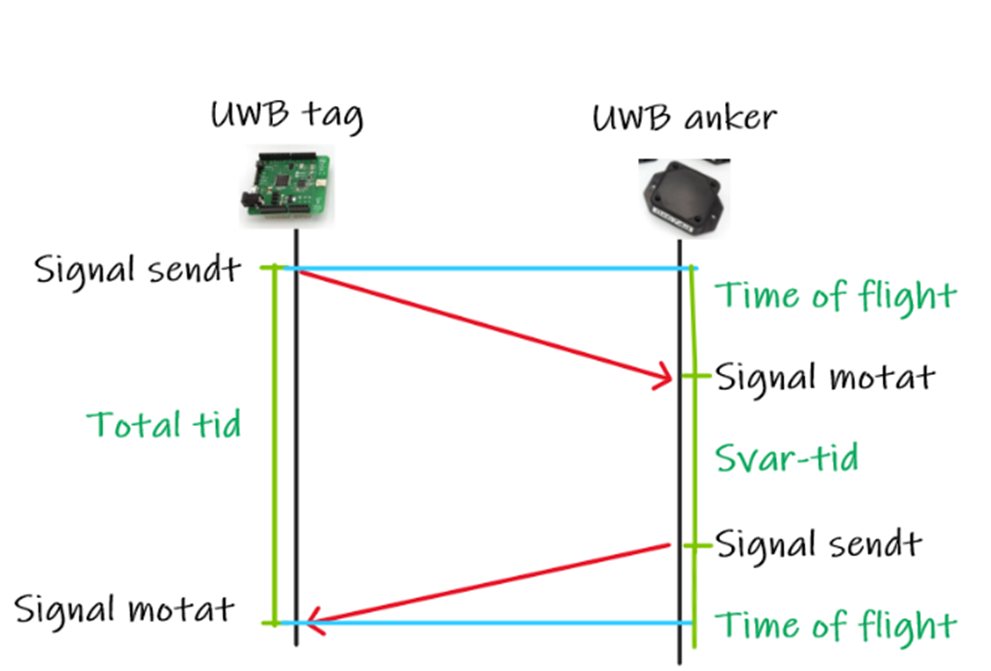
\includegraphics[width=0.7\columnwidth]{figures/twr}
    \caption{Two way ranging.}
    \label{fig:twr}
\end{figure}

For å finne avstanden mellom en tag og et anker brukes two way ranging (TWR) protokollen som vist i figur \ref{fig:twr}. 
Det man er ute etter å finne her er tiden signalet bruker fra ankeret til tagen, og bruke dette til å regne ut avstanden.
Et signal blir først sendt fra tagen til ankeret. Dette signalet bruker tiden $t_{of}$ (time of flight). 
Etter en viss tid, $t_{svar}$, sender ankeret et signal tilbake. Det antas at tiden fra tagen til ankeret er det samme som tiden fra ankeret til tagen, 
altså $t_{of}$. Når tagen mottar signalet tilbake fra ankeret regner den ut tiden fra den sendte ut signalet, 
til den fikk et signal tilbake ($t_{total}$). Dersom $t_{svar}$ er kjent på forhånd, 
kan man regne ut $t_{of}$ er dermed avstanden mellom tagen og ankeret:

\[t_{total} = t_{of} + t_{svar} + t_{of}\]
\[t_{total} = t_{svar} + 2 \cdot t_{of}\]
\[t_of = \frac{t_{total} - t_{svar}}{2}\]

UWB signalet reiser i lysets hastighet, altså: $v_{uwb} \approx 3 \cdot 10^8 m/s$

Dermed kan distansen regnes ut ved:\[d = t_{of} \cdot v_{uwb}\]


Grunnen til at TWR blir brukt er at det ikke krever synkronisering mellom tagen og ankeret. Så lenge $t_{svar}$ er kjent kan distansen regnes ut. 
Denne protokollen gjør også at det er tagen selv som regner ut distansen, 
som gjør det til en god protokoll for bruk på en drone som ønsker å vite sin egen posisjon. 
Det er også mulig å utvide TWR ved at tagen sender ut et ekstra signal etter den har fått signalet tilbake fra ankeret. 
På denne måten kan både tagen og ankeret regne ut avstanden mellom dem.
